% This is LLNCS.DOC the documentation file of
% the LaTeX2e class from Springer-Verlag
% for Lecture Notes in Computer Science, version 2.4
\documentclass{llncs}
\usepackage{llncsdoc}

% JobGraph fig
\usepackage{tikz}
\usetikzlibrary{arrows,automata,positioning,shapes.geometric}

% trademark symbol
\usepackage{textcomp}

\usepackage{float}

\newcommand{\TODO}[1]{\textcolor{red}{TODO: #1}}

% code listings
\usepackage{listings}

\newcommand{\sectionautorefname}{Section}%

\newcommand{\para}[1]{\vspace{2mm}\noindent\textbf{#1}}

\definecolor{dkgreen}{rgb}{0,0.6,0}
\definecolor{gray}{rgb}{0.5,0.5,0.5}
\definecolor{mauve}{rgb}{0.58,0,0.82}

% there is no built in support or Scala yet, good enough
\lstset{frame=l,
  language=Java,
  aboveskip=3mm,
  belowskip=3mm,
  showstringspaces=false,
  xleftmargin=5pt,
%   framexleftmargin=-1pt,
  columns=flexible,
  basicstyle={\scriptsize\ttfamily},
  numbers=none,
  numberstyle=\tiny\color{black},
  keywordstyle=\color{blue},
  commentstyle=\color{dkgreen},
  stringstyle=\color{mauve},
  breaklines=true,
  breakatwhitespace=true,
  tabsize=4,
  %for scala
  emph={%  
    object, def, val, zip, window, trigger, evict%
    },emphstyle={\color{blue}\textbf}%
}%

% url references
\usepackage{hyperref}

% in paragraph enums
\usepackage{paralist}

\usepackage{subfigure}

\def\definitionautorefname{Definition}
\def\sectionautorefname{Section}
\def\subsectionautorefname{Section}
\def\subsubsectionautorefname{Section}
\def\algorithmautorefname{Algorithm}
\def\figureautorefname{Figure}

\usepackage{amssymb}
\setcounter{tocdepth}{3}
\usepackage{graphicx}
\graphicspath{ {images/} }

\usepackage{url}
\newcommand{\keywords}[1]{\par\addvspace\baselineskip
\noindent\keywordname\enspace\ignorespaces#1}

\begin{document}

\mainmatter  % start of an individual contribution

% first the title is needed
\title{A Brief Overview of Apache Flink}
\subtitle{[Extended Abstract]}

% a short form should be given in case it is too long for the running head
\titlerunning{Apache Flink}

% the name(s) of the author(s) follow(s) next
%
% NB: Chinese authors should write their first names(s) in front of
% their surnames. This ensures that the names appear correctly in
% the running heads and the author index.
%
\author{Asterios Katsifodimos \and Volker Markl}
% \thanks{}
%

\authorrunning{Katsifodimos, Markl}
% (feature abused for this document to repeat the title also on left hand pages)

% the affiliations are given next; don't give your e-mail address
% unless you accept that it will be published
\institute{TU Berlin\\
\url{firstname.lastname@tu-berlin.de}
}


%
% NB: a more complex sample for affiliations and the mapping to the
% corresponding authors can be found in the file "llncs.dem"
% (search for the string "\mainmatter" where a contribution starts).
% "llncs.dem" accompanies the document class "llncs.cls".
%

\toctitle{Lecture Notes in Computer Science}
\tocauthor{Authors' Instructions}
\maketitle

\begin{abstract}
Apache Flink is an open source platform for scalable data processing. Flink's execution engine is based on a streaming dataflow engine, which serves both continuous data pipelines (stream) and historic data processing (batch). On top of its dataflow engine, Flink offers a set of APIs for creating applications, such as complex event processing (CEP), machine learning, and graph processing. In this extended abstract\footnote{This paper accompanies the invited talk given by Asterios Katsifodimos at the BIRTE Workshop (collocated with the VLDB conference) on August 31st, 2015.} we present a brief overview of the system, its libraries, and the main ideas behind its design.
\end{abstract}

\section{Introduction}
Apache Flink is an open source project licensed by the Apache Software Foundation (ASF), a non-profit organization that houses open source projects and their communities. Historically, Flink stems from the database research community, and in particular the Stratosphere research project \cite{stratosphere}. Flink entered the ASF in April 2014 as an “incubating” project, and “graduated” as a “top-level” project in December 2014. Since then, its community and contributors are increasing at  a fast pace, while Flink has been adopted by a number of web-scale companies.

Flink builds on the need of modern enterprises for timely, scalable, and efficient processing of large quantities of data. It incorporates and contributes novel ideas from stream processing, and database systems. In short, Flink offers: 
 \begin{itemize}
\item a paradigm for distributed dataflows based on the notions of operators and logical intermediate results.
\item a dataflow engine delivering low latency and high throughput.
\item efficient iterations within a DAG-based dataflow system \cite{DBLP:journals/pvldb/EwenTKM12}.
\item Cost-based optimization in the presence of user-defined functions \cite{battre2010nephele,blackBoxes}.
\item a novel technique for fault tolerant streaming computations with exactly-once guarantees \cite{carbone2015lightweight}.
\end{itemize}


This extended abstract is structured as follows. In \autoref{sec:overview}, we give an overview of the system and its user-facing libraries. In \autoref{sec:dataflows}, we give a brief description of the dataflow model implemented in Flink. We then describe the fault-tolerance mechanism in \autoref{sec:fault-tolerance} and conclude with the related work in \autoref{sec:related}.


\begin{figure}[t!]
\centering
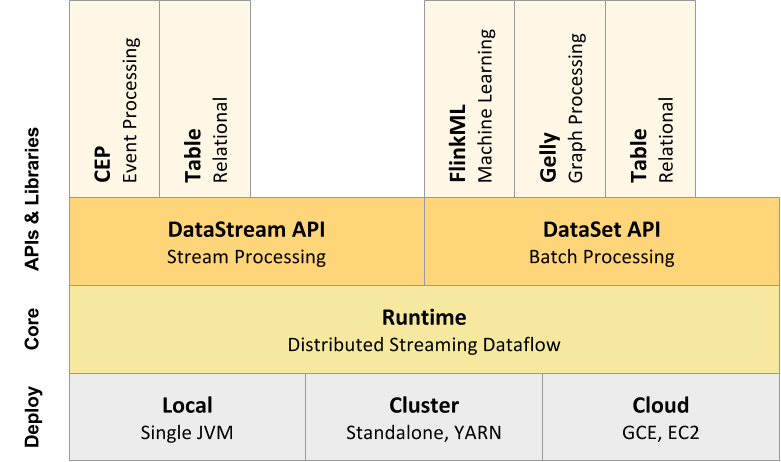
\includegraphics[width=.8\textwidth]{architecture}
\caption{Flink's Software Stack.}
\label{fig:stack}
\end{figure}

\section{System Overview}
\label{sec:overview}
Flink includes a number of APIs for creating applications on top of its streaming dataflow engine. At the top level (as seen in \autoref{fig:stack}) there are libraries for domain-specific use cases:
\begin{itemize}
\item \textbf{CEP}, a complex event processing library which enables applications such as infrastructure monitoring and alert generation for data centers by offering event pattern matching capabilities.
\item \textbf{Machine Learning} library, which facilitates the development of applications such as recommender systems (via matrix factorization, regression, etc.) by offering a set of supervised learning algorithm implementations.
\item \textbf{Gelly}, a graph processing API which offers a set of scalable graph analysis algorithm implementations, such as connected components detection, pagerank, etc. and provides a set of abstractions, which can be used to develop additional graph algorithms in a user-friendly manner.
\item \textbf{Table} API which offers a SQL-like expression language embedded in Java and Scala.
\end{itemize}

\noindent Flink's high-level abstractions and libraries are implemented on top of two lower-level APIs which enable programming streaming or batch dataflow programs. Those APIs are:
\begin{itemize}
    \item \textbf{DataStream} API for unbounded streams embedded in Java and Scala which provides means to partition, transform, join, define windows and aggregate data streams in parallel.
    \item \textbf{DataSet} API for static data embedded in Java, Scala, and Python which offers a set of transformations for parallel transformations such as map, reduce, join, etc. that can be applied on non-updating data sets.
\end{itemize}

All Flink programs that are written using high level libraries and APIs, are translated into programs which use a universal runtime implementing a distributed streaming dataflow model as described below.



\section{Streaming Dataflows}
\label{sec:dataflows}
The  dataflow  graph  depicted  in  \autoref{fig:dataflow-graph},  is  a  directed  acyclic  graph  (DAG)  that  consists  of:  (i)  stateful operators, and (ii) data streams that represent data produced by an operator and are available for consumption by operators. Since dataflow graphs are executed in a data-parallel fashion, operators are parallelized into one or more parallel instances called subtasks and streams are split into one or more stream partitions (one partition per producing subtask). The stateful operators implement the processing logic (e.g., filters, joins, window functions, and partitioners). 

\subsection{Stream Analytics on Top of Dataflows}
\begin{figure}[t!]
\centering
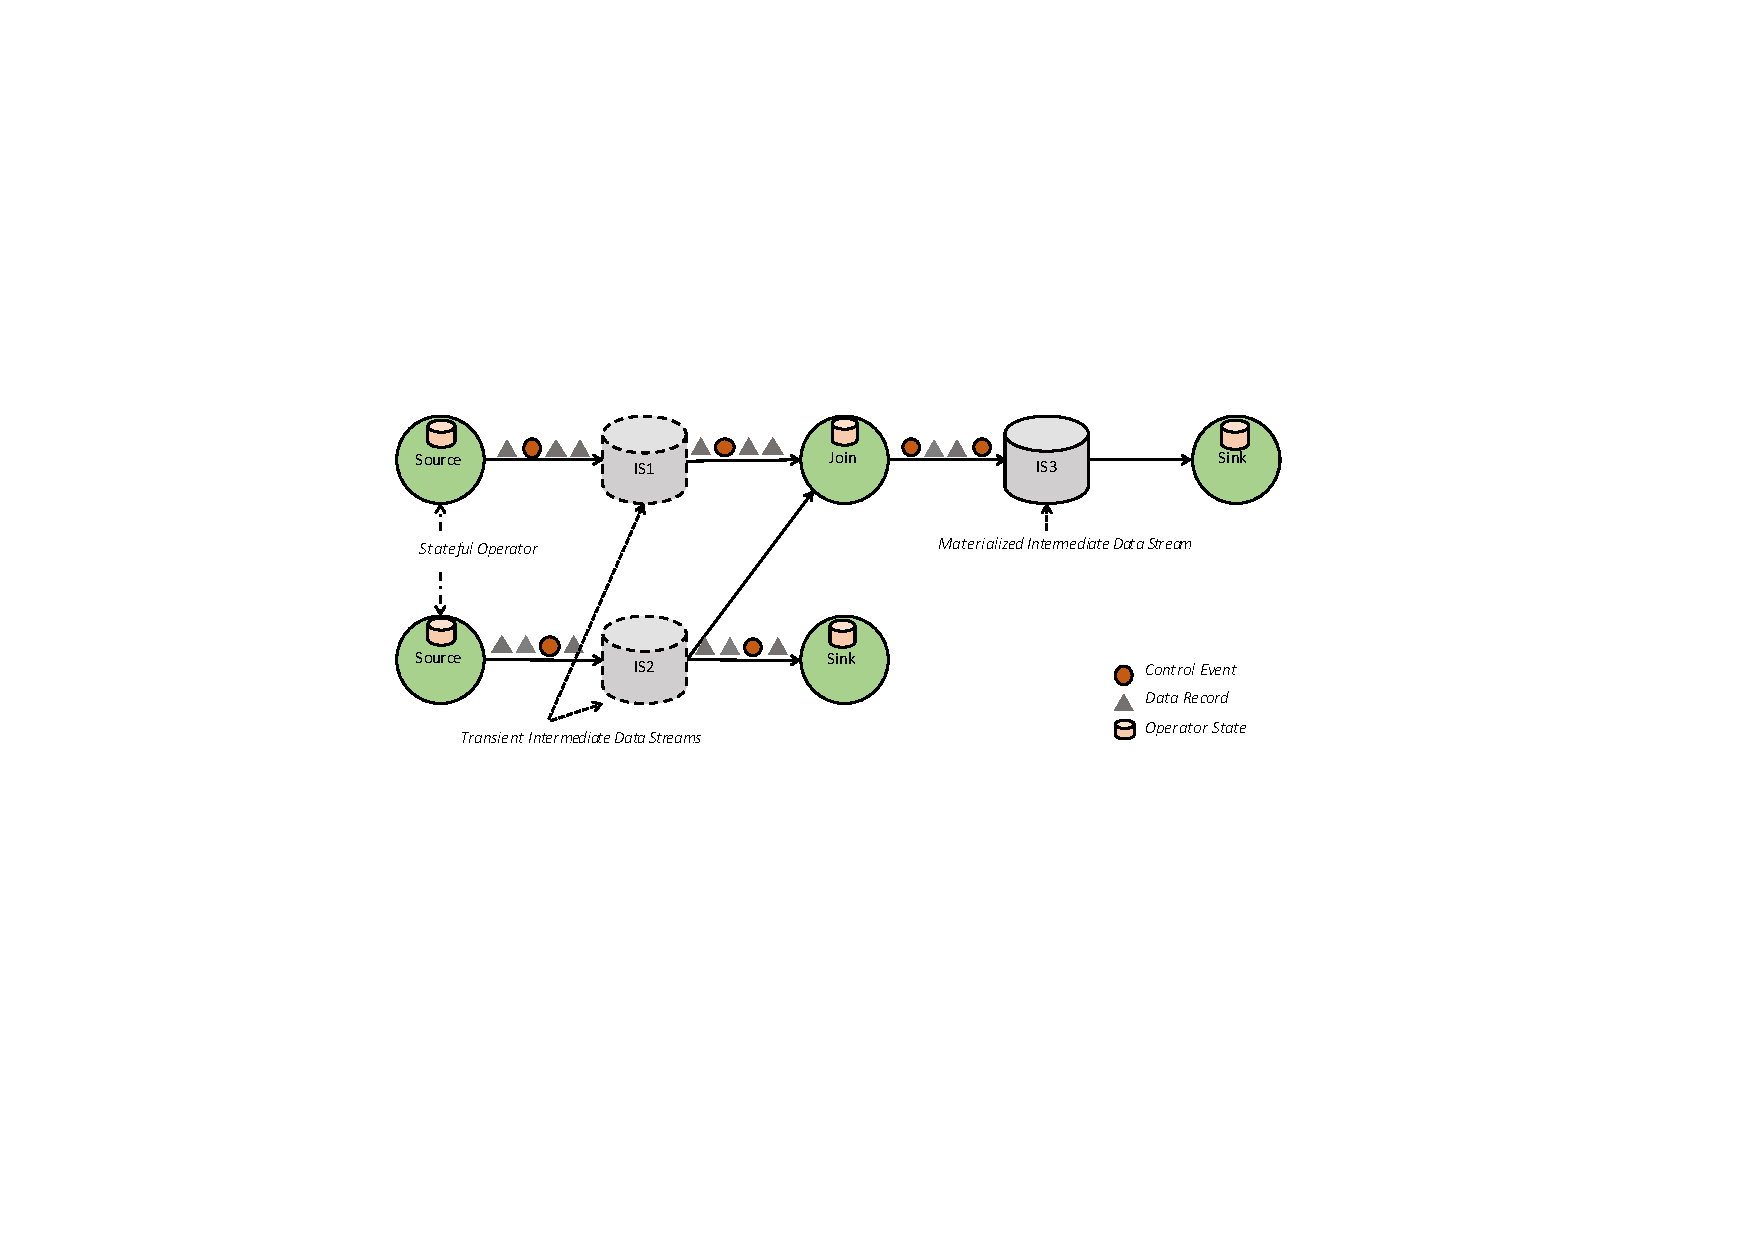
\includegraphics[width=.95\textwidth]{dataflow}
\caption{A Dataflow graph containing sources, sinks and a join operator.}
\label{fig:dataflow-graph}
\end{figure}

\subsubsection{Windows over Streams.}
Aggregating events, such as counts and sums works differently on streams than in batch processing. For instance, it is not possible to count \textit{all} elements in the stream and then return their count, since streams are, in principle, unbounded. Instead, aggregates on streams are performed over finite windows. Windows can be \textit{time driven} (e.g., window of 10 seconds) or \textit{data driven} (e.g., window of 10 elements). Flink implements different types of windows, such as tumbling, sliding, and session windows.

\subsubsection{Flink's Notion of Time.} Naturally, time-based windows require a notion of time. For instance, when defining a window one can take into account the current time of the machine in which the system is executing, and slice windows using the local system's clock. On the other hand, lots of applications are collecting and storing events outside the processing system (e.g., log files, Kafka topics). In these instances, the time on which the data was created is irrelevant to the time in which the data is actually being processed. To solve this issue, Flink offers its users three different notions of time upon which they can choose to implement their application:
\begin{itemize}
    \item \textbf{event time} i.e., the time when an event was created. It is usually described by a timestamp in the events, for example attached by the producing sensor, or the producing service. Flink accesses event timestamps via timestamp assigners.
    \item \textbf{ingestion time} i.e., the time when an event enters the Flink dataflow at the source operator.
    \item \textbf{processing time} i.e., the local time at each operator which performs a time-based operation.
\end{itemize}



\subsection{Batch Analytics on Top of Dataflows}
Flink treats batch processing as a special case of streaming. Batch programs are programmed over the DataSet API. In order to execute a batch program on top of a streaming dataflow, one has to bound the data streams, such that they emit a \textit{finite} number of elements. In case of failure, recovery happens by fully replaying the streams. This pushes the cost to the recovery mechanism, but makes the regular processing cheaper since it avoids checkpoints. Moreover, stateful operations in the DataSet API use in-memory/out-of-core data structures, rather than key/value indexes of the DataStream API. The DataSet API offers special synchronized iterations \cite{DBLP:journals/pvldb/EwenTKM12}, which are not possible in unbounded streams. Finally, Flink implements a set of optimizations \cite{blackBoxes}, which optimize the DAGs created with the Dataset API.


\vspace{-3mm}
\section{Fault Tolerance and Exactly-Once Stream Processing}
\label{sec:fault-tolerance}
Backing up and restoring the state of a computation is vital in the presence of software or infrastructure failures. On the event of such a failure, the system has to recover the state of the failed operator, and continue the computation, ideally,  from where it left off. As in transaction execution, different applications require different consistency guarantees. For instance, if no consistency guarantee is required (e.g., a live monitoring dashboard that displays clicks of a website), a system might simply recover the operator state to any previous snapshot and continue ingesting the stream. However, a computation that requires correctness of results (e.g., user interactions with their shopping basket) requires stricter consistency guarantees. 

\vspace{3mm}
\noindent The consistency guarantees provided by current streaming platforms include:
\begin{itemize}
\item \textbf{at most once} i.e., the fault tolerance mechanism does not guarantee anything (i.e.,  possibility for data loss). Apache Storm is one of the systems, which support at most once processing of streams
\item \textbf{at least once} i.e., the fault tolerance mechanism guarantees that an event is going to update the state of an operator at least once. In case of failure, some events of the stream might update the state multiple times. Systems implementing this consistency guarantee include Apache Storm and Apache Samsa
\item \textbf{exactly once} i.e., the operator state will be updated exactly once per event, no matter how many failures may happen. Here, execution under failures produces the same result as failure-free execution. Systems that implement this consistency guarantee include Apache Flink, Apache Spark, Millwheel, and Apache Storm (via the Trident micro-batch abstraction), etc.
\end{itemize}

In batch processing, guaranteeing exactly once consistency is relatively simple: the system simply pauses the computation, re-deploys (part of) the dataflow and re-consumes the necessary parts of its input. In the streaming case, however, i) computations are continuous (e.g., months of processing), ii) a data stream does not have, in principle, a beginning or an end, nor can it be stored indefinitely and iii) the computation cannot simply be stopped mid-flight.

Flink offers exactly once guarantees via a snapshot mechanism, which is based on an extension \cite{carbone2015lightweight} of the seminal Chandy-Lamport algorithm \cite{chandy1985distributed}. Flink's algorithm draws consistent snapshots of the current state of the distributed operators without missing information and without recording duplicates. Snapshots are taken asynchronously: the computation does not need to stop in order to take a snapshot. Flink’s fault tolerance mechanism draws state snapshots of a running stream topology, and stores these snapshots to durable storage (e.g., to HDFS or an in-memory file system). The frequency of these checkpoints can vary according to the failure rates and the cost of taking a snapshot.

\section{Related Work}
\label{sec:related}
The database community has produced a wealth of results in stream processing within projects like PSoup/Telegraph \cite{chandrasekaran2003psoup}, Aurora/Borealis~\cite{abadi2005design}, STREAM~\cite{arasu2004stream}, Trill~\cite{chandramouli2014trill} and IBM System S~\cite{gedik2008spade}. However, most of these systems either remained academic prototypes, or became closed-source products. Modern open source streaming systems, like Apache Storm and Samza, provide low level APIs, which enable DAGs of user-defined operators and offer at-least-once or at-most-once guarantees. MillWheel~\cite{akidau2013millwheel}, developed internally at Google, provides exactly-once guarantees with low latency. Millwheel is currently running Google Dataflow~\cite{akidau2015dataflow} programs. To the best of our knowledge, Flink is the only open-source project that offers high level APIs and processing libraries, exactly-once processing guarantees and serves both batch and streaming computations equally well. Apache Hadoop is the most popular open source system for batch processing of data and is based on the MapReduce paradigm~\cite{DBLP:journals/cacm/DeanG08}. Dryad~\cite{isard2007dryad}, introduced embedded user-defined functions in more general DAG-based dataflows and was used by SCOPE~\cite{scopeOptimizer}, which built an SQL optimizer on top of it. Apache Tez~\cite{saha2015apache}, an open source dataflow system has been highly influenced by Dryad. Parallel databases \cite{dewitt1990gamma}, as well as recent open-source implementations, like Apache Drill and Impala~\cite{kornacker2015impala} restrict their API to SQL variants. Similar to Flink, Apache Spark \cite{DBLP:conf/hotcloud/ZahariaCFSS10} implements a DAG-based processing framework, provides an SQL optimizer, and treats stream computations as micro-batches. In contrast, Flink:  
\begin{inparaenum}[i)]
  \item includes an optimizer that can optimize DAG programs beyond SQL queries,
  \item is able to perform very efficient native iterative processing,
  \item includes stream processing as a first-class citizen, thereby enabling lower latency in comparison to micro-batches.
\end{inparaenum}


\section{Acknowledgements}
The authors would like to thank Stefan Ewen, and Kostas Tzoumas  from data Artisans GmbH, Paris Carbone and Vasiliki Kalavri from KTH Stockholm, as well as the Flink community for their input concerning the content of this paper as well as for the slides they contributed to the invited talk.

\bibliographystyle{abbrv}
\bibliography{references}

\end{document}
